\documentclass[10pt,a4paper]{article}
\usepackage[utf8]{inputenc}
\usepackage[portuguese]{babel}
\usepackage{graphicx, hyperref, verbatim, multicol, amsmath, listings}

\addtolength{\oddsidemargin}{-1.4in}
\addtolength{\evensidemargin}{-1.4in}
\addtolength{\textwidth}{2.8in}
\addtolength{\topmargin}{-.875in}
\addtolength{\textheight}{1.75in}

\author{Grupo 47 \\\\ Daniel Fernandes 86400 \& \\Francisco Sousa 86416 \& Henrique Ferreira 86432}
\title{Projeto de Bases de Dados, Parte 4}
\begin{document}

\maketitle

\begin{center}
Turno BD22517957L09 \\
Sexta 12:30 Lab 8 \\
Prof. Taras Lykhenko \\
\end{center}

\begin{table}[h]
    \centering
    \begin{tabular}{lll}
    \hline
    \textbf{Número de Aluno} & \textbf{Nome} & \textbf{Esforço} \\ \hline
    86400 & Daniel Fernandes & 33\% (10h) \\ \hline
    86416 & Francisco Sousa & 33\% (10h) \\ \hline
    86432 & Henrique Ferreira & 33\% (10h) \\ \hline
    \end{tabular}
\end{table}
\newpage

\section{Restrições de Integridade}

Os mecanismos que achamos mais apropriados para a definição destas restrições
de integridade são os \underline{triggers}. Fazem consultas mais complexas do que o
\texttt{CHECK} e permitem lançar exceções.
Ainda, as operações com que trabalham não provocam \underline{triggers} em cadeia.

Assim, para cada problema, temos:

\paragraph{a)}
\begin{verbatim}
CREATE OR REPLACE FUNCTION chk_coord_local_on_solic_proc() 
RETURNS TRIGGER
AS $$
DECLARE morada_camara VARCHAR;
BEGIN
    SELECT morada_local INTO morada_camara FROM vigia WHERE num_camara = NEW.num_camara;
    IF EXISTS 
        (SELECT * FROM (audita NATURAL JOIN evento_emergencia) AS r
            WHERE r.morada_local = morada_camara
            AND r.id_coordenador = NEW.id_coordenador)
    THEN
        RETURN NEW;
    ELSE
        RAISE EXCEPTION 'Um coordenador so pode solicitar videos de camaras colocadas num local
        cujo accionamento de meios esteja a ser (ou tenha sido) auditado por ele proprio!';
        RETURN NULL;
    END IF;
END;
$$ LANGUAGE plpgsql;

DROP trigger IF EXISTS chk_coord_local_on_solic ON solicita;
CREATE trigger chk_coord_local_on_solic BEFORE INSERT ON solicita for each ROW EXECUTE procedure chk_coord_local_on_solic_proc();
    
\end{verbatim}

\paragraph{b)}
\begin{verbatim}
CREATE OR REPLACE FUNCTION chk_acciona_on_alocado_proc()
RETURNS TRIGGER
AS $$
BEGIN
    IF EXISTS
        (SELECT * FROM acciona
            WHERE num_meio = NEW.num_meio
            AND nome_entidade = NEW.nome_entidade
            AND num_processo_socorro = NEw.num_processo_socorro)
    THEN
        RETURN NEW;
    ELSE
        RAISE EXCEPTION 'Um Meio de Apoio so pode ser alocado a Processos de Socorro para
        os quais tenha sido accionado!';
        RETURN NULL;
    END IF;
END;
$$ LANGUAGE plpgsql;

DROP trigger IF EXISTS chk_acciona_on_alocado ON alocado;
CREATE trigger chk_acciona_on_alocado BEFORE INSERT ON alocado for each ROW EXECUTE procedure chk_acciona_on_alocado_proc();
    
\end{verbatim}
\section{Índices}

\paragraph{a)}
\subparagraph{Primeira Interrogação}
Os atributos verificados são \textit{num\_camara} na tabela \textbf{video} e \textit{num\_camara} e \textit{morada\_local} na tabela \textbf{vigia}.
Assim, para a tornar mais eficaz, fazemos dois índices:

O primeiro do tipo \underline{hash}, para \textit{num\_camara} na tabela \textbf{video}, pois lidamos com comparações entre números,
sendo agrupado e esparso.

O segundo do tipo \underline{balance tree}, para \textit{num\_camara} e \textit{morada\_local} na tabela \textbf{vigia}, sendo desagrupado e denso.

\subparagraph{Segunda Interrogação}
Perante o \texttt{GROUP BY}, torna-se adequado usar um índice \underline{balanced tree} composto para os atributos
\textit{num\_telefone} e \textit{instante\_chamada}.
São ainda criados outros dois índices \underline{hash} para \textit{num\_processo\_socorro}, tanto na tabela \textbf{transporta} como \textbf{evento\_emergencia},
para tornar mais eficaz a sua comparação, já que são variáveis únicas.

\paragraph{b)}
Assumindo que não existem quaisquer índices predefinidos sobre as tabelas, foram criados os seguintes:

\begin{verbatim}
\end{verbatim}

\section{Modelo Multidimensional}

O esquema em estrela é, representado na figura \ref{f1}, pode ser definido com as interrogações:

\begin{figure}[h]
	\centering
	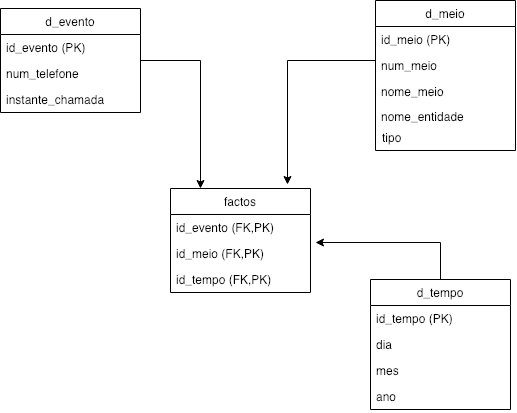
\includegraphics[width=0.5\textwidth]{modeloestrela}
	\caption{Esquema em estrela}
	\label{f1}
\end{figure}

\begin{verbatim}
drop table factos;
drop table d_evento;
drop table d_meio;
drop table d_tempo;

create table d_evento
    (id_evento serial,
    num_telefone char(9) not null,
    instante_chamada timestamp not null,
    constraint pk_id_evento primary key(id_evento)
);

create table d_meio
    (id_meio serial,
    num_meio char(5) not null,
    nome_meio varchar(255) not null,
    nome_entidade varchar(20) not null,
    tipo varchar(20) not null,
    constraint pk_id_meio primary key (id_meio)
);

create table d_tempo
    (id_tempo serial,
     dia int not null,
     mes int not null,
     ano int not null,
     constraint pk_id_tempo primary key(id_tempo)
);

create table factos
    (id_tempo int not null,
     id_meio int not null,
     id_evento int not null,
     constraint pk_factos primary key(id_tempo, id_meio, id_evento),
     constraint fk_tempo foreign key (id_tempo) references d_tempo(id_tempo),
     constraint fk_meio foreign key (id_meio) references d_meio(id_meio),
     constraint fk_evento foreign key (id_evento) references d_evento(id_evento)
);
\end{verbatim}

Usámos as seguintes queries para popular o esquema em estrela:

\begin{verbatim}
insert into d_evento (num_telefone, instante_chamada)
    select num_telefone, instante_chamada from evento_emergencia;

insert into d_meio (num_meio, nome_meio, nome_entidade, tipo)
    select num_meio, nome_meio, nome_entidade, 'apoio' from meio natural join meio_apoio;
insert into d_meio (num_meio, nome_meio, nome_entidade, tipo)
    select num_meio, nome_meio, nome_entidade, 'combate' from meio natural join meio_combate;
insert into d_meio (num_meio, nome_meio, nome_entidade, tipo)
    select num_meio, nome_meio, nome_entidade, 'socorro' from meio natural join meio_socorro;

insert into d_tempo (dia, mes, ano) values(22, 4, 2005);
insert into d_tempo (dia, mes, ano) values(15, 2, 2009);
insert into d_tempo (dia, mes, ano) values(29, 2, 2018);
insert into d_tempo (dia, mes, ano) values(27, 8, 1998);
insert into d_tempo (dia, mes, ano) values(28, 8, 1996);
insert into d_tempo (dia, mes, ano) values(1, 10, 1999);
insert into d_tempo (dia, mes, ano) values(7, 8, 1997);
insert into d_tempo (dia, mes, ano) values(27, 1, 1999);
insert into d_tempo (dia, mes, ano) values(3, 7, 2007);
insert into d_tempo (dia, mes, ano) values(3, 9, 2018);
insert into d_tempo (dia, mes, ano) values(9, 8, 1998);
insert into d_tempo (dia, mes, ano) values(4, 7, 2000);
insert into d_tempo (dia, mes, ano) values(11, 9, 2001);
insert into d_tempo (dia, mes, ano) values(24, 7, 2015);

insert into factos
    select id_tempo, id_meio, id_evento from d_evento cross join d_meio cross join d_tempo;
\end{verbatim}

\section{Data analytics}

Considerando o esquema em estrela criado anteriormente, fizemos duas interrogações
SQL OLAP para obter o número de meios de cada tipo utilizados no evento número 15, com
rollup por ano e mês. Ambas mostram o número de meios ordenados por cada um dos critérios
\textit{mes}, \textit{ano}, \textit{tipo}, em ordem ascendente, listando a soma dos tipos,
tanto por mês, como por ano, como por tipo.

Para versão de postgres inferior a 9.5, usamos \texttt{UNION}:

\begin{verbatim}
select tipo, ano, mes, count(*)
    from (d_tempo natural join d_meio natural join
        (select * from factos where id_evento = '15') as a) 
    group by tipo, ano, mes
union
select tipo, ano, null, count(*) 
    from (d_tempo natural join d_meio natural join
        (select * from factos where id_evento = '15') as a) 
    group by tipo, ano
union
select tipo, null, null, count(*) 
    from (d_tempo natural join d_meio natural join
        (select * from factos where id_evento = '15') as a) 
    group by tipo
union
select null, null, null, count(*) 
    from (d_tempo natural join d_meio natural join
        (select * from factos where id_evento = '15') as a)
order by tipo, ano, mes;
\end{verbatim}

Usando \texttt{ROLLUP}, para versão postgres igual ou superior a 9.5:

\begin{verbatim}
select tipo, ano, mes, count(*)
    from (d_tempo natural join d_meio natural join
    (select * from factos where id_evento = '15') as a)
group by rollup (tipo, ano, mes)
order by tipo, ano, mes;
\end{verbatim}



\end{document} 